





%==============================================
\subsection{Weighted Average Flux (WAF) Method}\label{chap:hydro-WAF}
%==============================================







%============================================
\subsubsection{Method}
%============================================


For the WAF method, we again assume piece-wise constant data (see fig. \ref{fig:piecewise-constant}), i.e.

\begin{equation}
	\U_i ^ n = \frac{1}{\Delta \x} \int_{\x_{i-\half}}^{\x_{i+\half}} \U(\x, t^n) \de \x
\end{equation}

The scheme is again based on the explicit conservative formula

\begin{equation}
	\U_{i}^{n+1} = \U_i^n + \frac{\Delta t}{\Delta x} \left[ \F_{i - \half} - \F_{i + \half} \right] \label{eq:hydro_basics_waf}
\end{equation}



The intercell flux $\F_{i + \half}$ is defined as an integral average of the flux function:

\begin{equation}
	\F_{i + \half} = \frac{1}{\Delta x} \int_{-\frac{1}{2} \Delta x} ^{\frac{1}{2} \Delta x} \F (\U_{i+\half} ( x, \frac{1}{2}\Delta t)) \de x \label{eq:hydro-waf-flux}
\end{equation}

The integration range goes from the middle of the cell to the middle of the neighbouring cell.





\begin{figure}[htbp]
	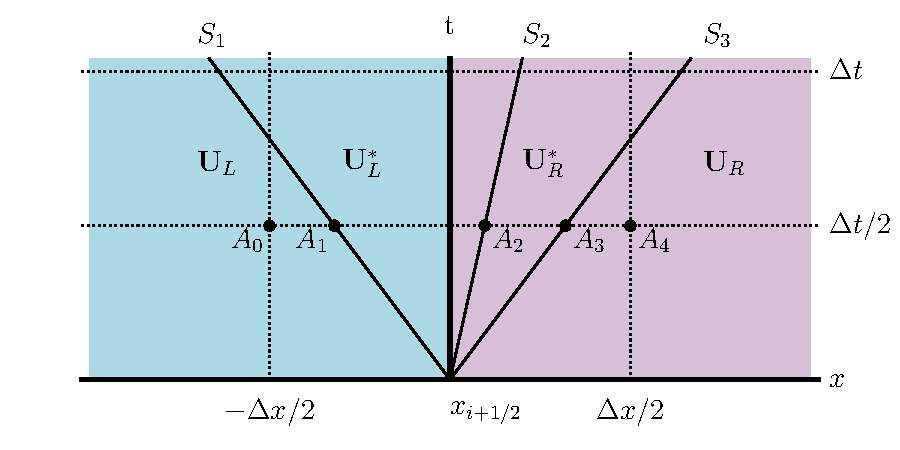
\includegraphics[width=\textwidth]{./figures/WAF-hydro.pdf}%
	\caption{Figure to show the derivation of the WAF intercell flux (eq. \ref{eq:hydro-waf-flux}) for the 1D Euler equations.
		We have initially two piecewise constant states, $\U_i$ and $\U_{i+1}$, separated at the position $x_{i+\half}$.
		As time evolves, three waves will emerge, with respective speeds $S_1$, $S_2$, and $S_3$.
		The states between the points $A_k$, $A_{k+1}$ are assumed constant.
		\label{fig:hydro-waf}
	}
\end{figure}



The solution of the Riemann problem separates the two initial states $\U_L = \U_i$, $U_R = \U_{i+1}$ into four states

\begin{align*}
	\U^{(1)} = \U_L, \quad	\U^{(2)} = \U_L^*, \quad	\U^{(3)} = \U_R^*, \quad	\U^{(4)} = \U_R
\end{align*}

that are separated by three waves with the speeds $S_1$, $S_2$, and $S_3$.
At $t = \frac{1}{2} \Delta t$, we can separate the interval $[-\Delta x /2, \Delta x /2]$ by introducing 5 points along the $x$ axis:

\begin{align*}
	A_0 &= - \Delta x / 2\\
	A_1 &= S_1 \Delta t / 2\\
	A_2 &= S_2 \Delta t / 2\\
	A_3 &= S_3 \Delta t / 2\\
	A_4 &= \Delta x / 2
\end{align*}

and separate the integral \ref{eq:hydro-waf-flux} into the sum
\begin{align}
\F_{i + \half} = \frac{1}{\Delta x} \sum\limits_{k = 1}^{N+1} \int\limits_{A_{k-1}}^{A_k} \F (\U(x, \Delta t / 2)) \de x
\end{align}

where $N$ is the number of occuring waves in the solution.





Note that with $|C_{cfl}| \leq 1$ we should always have all the waves within $[-\Delta x /2, \Delta x / 2]$ at $t = \Delta t / 2$ if the $C_{cfl}$ is chosen properly using actual wave speeds.
However, we use approximate wave speed estimates, so we need to check whether the actual waves are still inside $[-\Delta x /2, \Delta x / 2]$ at $t = \Delta t / 2$.



Since we assume constant states between these points (which they will be unless we have a rarefaction present), the fluxes $\F$ between the points $A_k$ will be constant too, and the integral is trivial.
We only need expressions for the distances $\overline{A_{k}A_{k+1}}$.
It's easy to show that regardless of the sign of the wave speeds $S_k$, we obtain

\begin{align*}
	\overline{A_0 A_1} &= 
		\frac{\Delta x}{2} ( 1 + c_1 ) \\
	\overline{A_1 A_2} &= 
		\frac{\Delta x}{2} ( c_2 - c_1 ) \\
	\overline{A_2 A_3} &= 
		\frac{\Delta x}{2} ( c_3 - c_2 ) \\
	\overline{A_3 A_4} &= 
		\frac{\Delta x}{2} ( 1 - c_3 ) \\ 
	\text{ with } c_k &= \frac{S_k \Delta t}{\Delta x}
\end{align*}



If we define

\begin{align*}
	\beta_k &= \frac{\overline{A_{k-1} A_k}}{\Delta x}\\
	c_0 &= -1, \quad c_5 = c_{N+1} = 1
\end{align*}

we obtain

\begin{align*}
	\beta_k &= \frac{1}{2} (c_k - c_{k-1})
\end{align*}

and we can write the WAF flux as

\begin{align}
	\F_{i + \half} 
		&= \sum\limits_{k = 1}^{N+1} \beta_k \F^{(k)} \\
		&= \frac{1}{2} (\F_i + \F_{i+1}) - \frac{1}{2} \sum\limits_{k = 1}^{N} c_k \left (\F^{(k+1)} - \F^{(k)} \right) 
\end{align}




The TVD modification of the WAF flux is


\begin{align}
	\F_{i + \half} 
		&= \frac{1}{2} (\F_i + \F_{i+1}) - \frac{1}{2} \sum\limits_{k = 1}^{N} sign(c_k) \psi_{i+\half}^{(k)} \left (\F^{(k+1)} - \F^{(k)} \right) \\
	\psi_{i+\half}^{(k)}
		&= \psi_{i+\half}(r^{(k)}) \\
	r^{(k)} &=
		\begin{cases}
			\frac{\Delta q_{i-\half}^{(k)}}{\Delta q_{i+\half}^{(k)}}	& \text{ if } c_k > 0 \\[2em]
			\frac{\Delta q_{i+3/2}^{(k)}}{\Delta q_{i+\half}^{(k)}}	& \text{ if } c_k < 0 \\		
		\end{cases}
\end{align}

Where $q$ is one single quantity which is known to change across every wave.
Options are density $\rho$ and internal energy $\epsilon$.
I implemented the choice $\rho$.

The notation here is a bit tricky: $k$ signifies which wave in the solution of Riemann problems (not only one Riemann problem!!) we look at:

\begin{itemize}
	\item $\Delta q_{i+\half}^{(k)}$ is the jump in e.g. density between wave $k$ and $k + 1$ of the solution of the Riemann problem with initial conditions $\U_L = \U_i$, $\U_R = \U_{i+1}$
	\item $\Delta q_{i-\half}^{(k)}$ is the jump between wave $k$ and $k+1$ of the solution of the Riemann problem with initial conditions $\U_L = \U_{i-1}$, $\U_R = \U_{i}$
	\item $\Delta q_{i+3/2}^{(k)}$ is the jump between wave $k$ and $k+1$ of the solution of the Riemann problem with initial conditions $\U_L = \U_{i+1}$, $\U_R = \U_{i+2}$
\end{itemize}

See figure \ref{fig:WAF-delta-q} for visual clarification.



\begin{figure}[htpb]
	\centering
	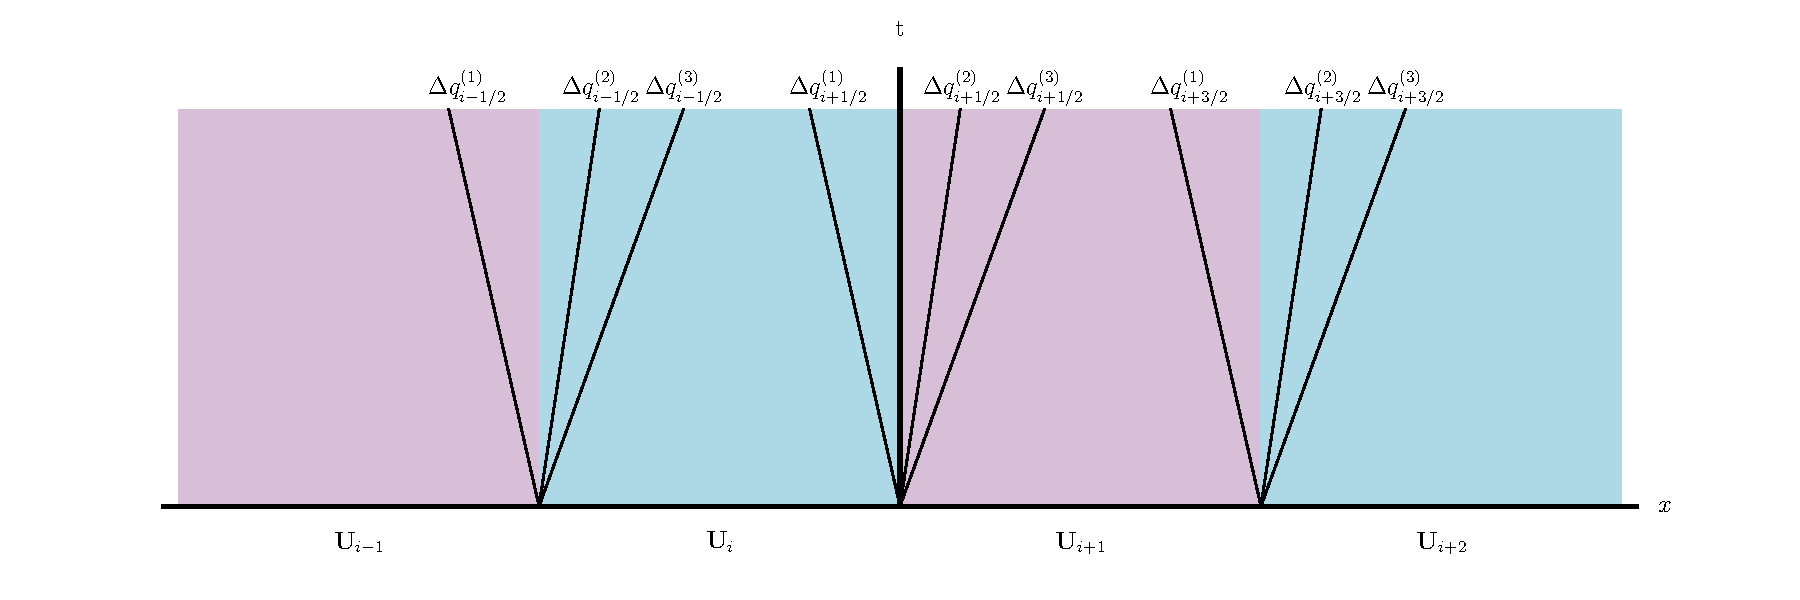
\includegraphics[width=\textwidth]{figures/WAF-hydro-delta-q.pdf}%
	\caption{
		Clarification of the value differences $\Delta q _{i}^{(k)}$ needed to compute the flow parameter $r$ for the WAF method.
		\label{fig:WAF-delta-q}
	}
\end{figure}



The limiters $\psi$ are related to conventional flux limiters $\phi$ via

\begin{equation}
	\psi_{i+\half} = 1 - ( 1 - |c|) \phi_{i+\half}(r)
\end{equation}

Some implemented options are given in section \ref{chap:implemented_limiters}.












%===================================================================
\subsubsection{Dealing with Vacuum}\label{chap:hydro-WAF-vacuum}
%===================================================================


Vacuum needs some special attention because it doesn't follow the solution structure of a typical Riemann problem.
It can easily crash your program:
Consider for example the computation of the local sound speed $a = \sqrt{\gamma p/\rho}$ for $\rho = 0$.
There is no more star region present, instead next to the vacuum ($\rho = 0$) we have a contact wave coinciding with the tail of a rarefaction wave - a wave that we also handle only approximately.

I wasn't able to find literature of how to best deal with this, but I was able to find an approximate solution on my own following the idea of how the WAF scheme works.

In the end, what we want is a solution that we can use to get WAF fluxes, namely we need

\begin{itemize}
	\item 4 fluxes $\F_{i}^{(k)}$ corresponding to the four states $\U_{i}^{(k)}$: $U_L$, $U_L^*$, $U_R^*$, $U_R$
	\item 3 wave speeds $S_L$, $S^*$, $S_R$
	\item 3 differences/jumps in density $q^{(k)}$: $\rho_L^* - \rho_L$, $\rho_R^* - \rho_L^*$, $\rho_R - \rho_R^*$
\end{itemize}

For vacuum, we have three cases to consider, where $\U_{vac}$ describes the vacuum state:


\begin{enumerate}

	\item 	\textbf{The right state is a vacuum}:
	
			Choose 
			\begin{align*}
				\F^{(1)} &= \F(\U_L)\\
				\F^{(2)} &= \begin{cases}
								&\F(\U(t = \Delta t/2, \ x = 0) \quad \text{ for a sonic rarefaction } \\
								&\F(\U_L) \quad \text{ for a non-sonic rarefaction } \\
							\end{cases}\\
				\F^{(3)} &= \F(\U_{vac})\\
				\F^{(4)} &= \F(\U_R)\\[.5em]
				S^{(1)} &= 0\\
				S^{(2)} &= \text{ rarefaction tail speed}\\
				S^{(3)} &= \text{ rarefaction head speed}\\[.5em]
				q^{(1)} &= \rho^*_L - \rho_L\\
				q^{(2)} &= 0\\
				q^{(3)} &= 0\\							
			\end{align*}
			
			Where $\rho^*_L$ is either the density of $\U_L$ or of $\U(x = 0, t = \Delta t/2)$, depending on whether we have a sonic or non-sonic rarefaction.

	
	\item 	\textbf{The left state is a vacuum}:
			
			Choose 
			\begin{align*}
				\F^{(1)} &= \F(\U_L)\\
				\F^{(2)} &= \F(\U_{vac})\\
				\F^{(3)} &= \begin{cases}
								&\F(\U(t = \Delta t/2, \ x = 0) \quad \text{ for a sonic rarefaction } \\
								&\F(\U_R) \quad \text{ for a non-sonic rarefaction } \\
							\end{cases}\\
				\F^{(4)} &= \F(\U_R)\\[.5em]
				S^{(1)} &= 0\\
				S^{(2)} &= \text{ rarefaction tail speed}\\
				S^{(3)} &= \text{ rarefaction head speed}\\[.5em]
				q^{(1)} &= 0\\
				q^{(2)} &= 0\\
				q^{(3)} &= \rho_R - \rho_R^*\\							
			\end{align*}
			
			Where $\rho^*_R$ is either the density of $\U_R$ or of $\U(x = 0, t = \Delta t/2)$, depending on whether we have a sonic or non-sonic rarefaction.
			
	
	\item 	\textbf{A vacuum is being generated}:
	
			This may occur when condition \ref{eq:vacuum-generating-condition} is satisfied.
			The solution structure contains two rarefaction fans, to the left and to the right, enclosed by the initial states $U_L$ and $U_R$, and separated by a vacuum state $U_{vac}$.
			
			My solution strategy is as follows:
			Compute an approximate solution to describe the average state inside each rarefaction fan, and then ``stretch'' the states out such that we pretend that there is no vacuum state in between.
			
			For example, for the left star state, we can compute the rarefaction head speed $S_{L,H}$ and tail speed $S_{L,T}$ and define the average speed $\overline{S}_L = \frac{S_{H,L} + S_{T,L}}{2}$.
			
			Now we approximate the entire star state as the solution inside a rarefaction fan, eqns. \ref{eq:rho-rarefaction-fan-left}-\ref{eq:pressure-rarefaction-fan-left} and \ref{eq:rho-rarefaction-fan-right}-\ref{eq:pressure-rarefaction-fan-right}, at $x/t = \overline{S}_L$.
			The same computation can be done for the right rarefaction.
			
			Then we say that we have no vacuum state in between, but instead ``stretch out'' the star states to meet at a contact wave with speed $S^* = \frac{S_{T,L} + S_{T,R}}{2}$.
			However, we want the total mass, momentum, and energy to be conserved.
			Hence we need to reduce the density, momentum, and energy by a factor
			\begin{align*}
				f_{L,R} = \frac{S_{HL,R} - S_{L,R}}{S_{HL,R} - \frac{S_L + S_R}{2}}
			\end{align*}
			which is simply the ``stretch factor'' based on the distances the utilized waves would travel at any given time $t > 0 $.
			
			In terms of primitive variables, it suffices to apply this factor to density and pressure such that energy, momentum, and mass conservation are satisfied.
			With this, we have expressions for the two star states and a contact speed $S^*$, and can now easily compute the four necessary fluxes.
			
			This solution is not very good, because even when applying flux limiters, it will introduce new peaks at the position of the vacuum.
			However, due to the lack of a better idea, this is what we have.
			At least it provides a somewhat usable solution, such that the WAF method can be used in actual hydrodynamics applications without worrying of code crashes should such a condition occur even for very small time steps.
			

\end{enumerate}
























%===================================================================
\subsubsection{Implementation Details}\label{chap:hydro-WAF-details}
%===================================================================



The cells are stored just like in the Godunov method.
Additionally, we need to store

\begin{itemize}
	\item the three wave speeds $S^{(1)}$, $S^{(2)}$, $S^{(3)}$ as \texttt{float}s
	\item the four fluxes in the four constant regions $\F_L$, $\F_L^*$, $\F_R^*$, $\F_R$ (in that order) as \texttt{cstate}s
	\item the three jumps in density $\Delta q^{(1)}$, $\Delta q^{(2)}$, $\Delta q^{(3)}$ between each wave
\end{itemize}

for each cell.


The flux at $x_{i+\half, j}$ and $y_{i, j+\half}$ are stored in \texttt{cflux}of cell \verb|grid[i, j]|.
Because we're doing dimensional splitting, it suffices to have only one storage place, as they will be used in successive order.
See section \ref{chap:dimensional-splitting} for details.

We can afford to store $x_{i+\half}$ at cell $i$ because we have at least 2 extra virtual boundary cell which is used to apply boundary conditions, so the flux at $x_{-\half}$ will be stored in \verb|grid[BC-1]|, where \texttt{BC} is the number of boundary cells used, defined in \texttt{defines.h}.
 



The related functions are written in \texttt{/program/src/solver/waf.c} and \texttt{/program/src/solver/waf.h}.
The hydro related functions are called in the main loop in \texttt{/program/src/main.c} when \verb|solver_step(...)| is called.

The \verb|solver_step(...)| function does the following for the 1D case:
\begin{itemize}
	\item 	Reset the stored fluxes from the previous timestep to zero
	\item 	Compute the primitive states for all cells from the updated conserved states
	\item 	Impose boundary conditions (section \ref{chap:boundary-conditions})
	\item 	Find the maximal timestep that you can do by applying the CFL condition \ref{eq:godunov-cfl}.
	\item 	Compute fluxes:
	\begin{itemize}
		\item 	For every cell, first solve the Riemann problem and find the three wave speeds, four fluxes, and three jumps in density.
				We need all the jumps in density present before we can compute the fluxes, because for the limiting procedure, the $k$-th wave of cell $i$ is compared to the $k$-th wave of cells $i \pm 1$.
				Hence all the waves between all pairs of cells need to be known before the actual intercell flux can be computed.
				This is done by first solving the Riemann problems between each cell pair in a single loop over all cells, and then the rest of the solution is done in a second loop over all cells.
		\item 	For every cell pair, compute the WAF flux using the wave speeds, jumps over density, and fluxes found in the previous loop.
		\item 	Store the flux $\F_{i+\half}$ in the \texttt{struct cstate cflux} struct of the cell $i$.
	\end{itemize}
	\item 	Update the states: Effectively compute $\U^{n+1}$ at this point using $\U_i^n$, the flux $\F_{i+\half}$ stored in every cell $i$, and the flux $\F_{i-\half}$ stored in every cell $i-1$.
\end{itemize}



